\documentclass[11pt, a4paper]{article}

\usepackage{amssymb}
\usepackage{bm}
\usepackage{mathtools}
\usepackage{centernot}
\usepackage[]{algorithm2e}
\usepackage{amsmath}
\usepackage{graphicx}
\usepackage{subcaption}
\usepackage{wrapfig}
\usepackage{lipsum}
\usepackage{url}
\usepackage{array}
 
\graphicspath{{./images/}}
		
\newcommand{\matr}[1]{\bm{\mathit{#1}}}

\title{Detecting Sources of Misinformation in Social Networks using Advantage Actor Critic}
\author{Johannes Cox, Student-ID: 408443}

\begin{document}
	
\maketitle

\section{Introduction}

\section{Modeling the Social Network} \label{sec:SN}
The social network contains a finite set of members $\mathbb{V}$ with $|\mathbb{V}| = N$. Each member has a belief at time $t$, the beliefs of all members at time $t$ is defined as $\vec{b}(t)$. Each belief is in the range $[0,1]$, that is 
%
\begin{equation}
\vec{b}_i(t) \in [0,1] \ \ \ \forall i = 1,...,N \ .
\end{equation}
%
Therefore, the belief $\vec{b}_i(t)$ can be interpreted as the belief of a member about a certain thesis where $	\vec{b}_i(t) = 0$ means that the person fully disagrees, $\vec{b}_i(t) = 1$ means that the person fully agrees and $\vec{p}_i(t) = 0.5$ means that the person is indifferent to the thesis. It is also possible to interpret the beliefs $\vec{b}_i(t)$ as the person's opinion about a certain topic. It can be applied to topics in which it is possible to order opinions in a continuous way such that $\vec{b}_i(t) = 0$ corresponds to an extreme opinion and $\vec{p}_i(t) = 1$ corresponds to an opposed extreme opinion whereas $\vec{b}_i(t) = 0.5$ is an opinion in between. \newline

The social network is modeled as a directed graph where a node corresponds to a member of the network and an edge corresponds to a connection between two members. The edges are drawn randomly with a method proposed by Gilbert \cite{random_graphs} where an edge between two nodes is created with probability $p_{e}$. Hence, it is expected that the graph contains $\frac{p_{e}N(N-1)}{2}$ edges and nodes have $p_{e}\cdot N$ neighbors on average.\newline

The exchange of information in the proposed network can be seen as a mixture between Naive Learning \cite{NaiveLearning1,NaiveLearning2,NaiveLearning3} and a model where members are influenced by external sources; similar to models which are for instance used to describe viral marketing \cite{viral_marketing1, viral_marketing_2, viral_marketing_3}. The new belief vector $\vec{b}(t)$ at iteration $t$ can be calculated by taking the sum of two factors. The first factor is called network factor and is defined as 
%
\begin{equation}
	\vec{b}_\text{network}(t) = \matr{H} \vec{b}(t-1)
\end{equation} 
%
which corresponds to the update rule of naive learning. $\matr{H} \in \Re^{IxI}$ is a stochastic matrix, thus, every row of $\matr{H}$ sums to $1$. Furthermore, $\matr{H}_{ij} \neq 0 \Leftrightarrow \matr{A}_{ij} = 1$ with $\matr{A}$ being the adjacency matrix of the graph. Therefore, $\matr{H}_{ij}$ can be interpreted as how much a person $i$ trusts person $j$. In the following the trust values $\matr{H}_{i}$ are uniformly distributed over all neighbors of $i$ for simplicity. \newline
The second factor is called source factor and describes the influence of external sources onto the members of the network. External sources can be interpreted as media channels like television, radio, blogs and so on. In the case of a source that propagates a false belief value it is also possible to interpret that as a bot network where the source controls the belief value of the nodes that have full trust into that specific source. The source factor is defined as
%
\begin{equation}
	\vec{b}_\text{source} = \matr{T} \vec{s}+\eta
\end{equation}
%
where $\vec{s}$ includes all external sources with $\vec{s}_i \in [0,1]$ and $\matr{T}_{ij}$ corresponds to how much a person $i$ trusts a source $j$. Gaussian white noise is added with the term $\eta \sim \mathcal{N}(0,\sigma)$. Matrix $\matr{T}$ is also a stochastic matrix. Note that the source factor is constant over all iterations. It is assumed that there are sources that propagate a true belief value $s_T \in [0,1]$ and sources that propagate a random false belief value $s_F$. The true source value $s_T$ is drawn by a uniform distribution within the interval $[0,1]$ and the false source values are drawn by a uniform distribution within the intervals $[0, s_T-0.3]$ and $[s_T+0.3,1]$. This guarantees that the false sources propagate a belief value that deviates from the true value by at least $0.3$. For simplicity it is assumed that every member of the network only has a nonzero trust value to one external source.\newline

The belief vector $\vec{b}(t)$ at iteration $t$ can thus be calculated as
%
\begin{equation} \label{equ:update}
\vec{b}_i(t) = \vec{\delta}_i \matr{H}_i \vec{b}(t-1) + (1-\vec{\delta}_i)\matr{T}_i \vec{s}+\eta
\end{equation}
%
with $\vec{b}(0) = \matr{T} \vec{s}+\eta$. The vector $\vec{\delta}$ corresponds to how much the members of the social network trust the beliefs that are propagated in the network and in the external sources respectively. The update rule in equation (\ref{equ:update}) can be seen as an extension of naive learning where external sources influence the beliefs and false information is spreading through the network. \newline

\section{Social Network Model as a Reinforcement Learning Environment} \label{sec:SN_RLEnv}
The model that was introduced in section (\ref{sec:SN}) is now extended such that it can act as an environment for reinforcement learning. In order to achieve that an observation space, an action space and a reward function has to be defined.

\subsection{Observation Space}
The observation space $\mathcal{O}$ consists of the belief values of all members of the network as well as the current iteration divided by the number of maximum iterations $T$ which gives a feedback of how much iterations are left. The observation $o$ at iteration $t$ is
\begin{equation}
o(t)=[\frac{t}{T},\vec{b}_1(t),...,\vec{b}_{N}(t)]
\end{equation}
Therefore, $\mathcal{O} \in \Re^{N+1}$ and $\mathcal{O}_i \in [0,1] \, \forall i \in 0...N$. This means that the environment has a continuous observation space whose dimensionality increases linear with the number of members in the social network. \newline
Note that the exact topology of the network is not passed to the agent. Thus, the agent has to detect misinformation without exact knowledge of how the members in the network are connected to each other.

\subsection{Action Space}
At each iteration the agent has to determine how much the belief of each social network member can be trusted. This is achieved by assigning a number in the interval $[0,1]$ to each member whereat a value of $0$ corresponds to no trust and $1$ corresponds to full trust. All members with a trust smaller than $0.1$ are excluded from the network, that is if action $a_i<0.1$ entries $\matr{H}_{ij}$ and $\matr{H}_{ji}$ $\forall j \in [1,N]$ are set to $0$. \newline
Defining the action space in a continuous way allows to not only determine wether a member of the social network is trustworthy or not but also to what degree. As a downside this leads to a large action space which makes it more challenging to train an agent with reinforcement learning \cite{large_action_2,large_action_1}.

\subsection{Reward Function}
Finding a suitable reward function is a crucial challenge in most reinforcement learning applications \cite{reward_design_1,reward_design_2}. The reward function has to precisely define the goal the agent should achieve. Furthermore, the design of the reward function is an important component to prevent getting stuck in local minima during training. \newline
We want to determine the level of misinformation for each member in the network while also excluding members who spread misinformation to a high degree such that the average belief in the network can converge to the true source value $s_T$ similar to naive learning \cite{NaiveLearning1}. The following term defines the estimated true source value $\overline{s}_{\text{est}}$ where the belief values of all non-excluded members $\vec{b}_{\text{active}}(t)$ is scaled by the trust given by action $a(t)$.
%
\begin{equation} \label{equ:s_est}
	\overline{s}_{\text{est}}(\vec{a}(t))=\frac{1}{\sum_{i}^{}\vec{a_i}(t)} \vec{a(t)} \cdot \vec{b}_{\text{active}}(t)
\end{equation}
%
The environment then returns a reward based on how far this estimated source value deviates from the real one.
%
\begin{equation}
	r(\vec{a})= \begin{cases}
		0 & \text{all members are excluded}\\
		0 & |s_T-\overline{s}_{\text{est}}|>0.5\\
		1-2 \cdot |s_T-\overline{s}_{\text{est}}| & \text{otherwise}
	\end{cases}
\end{equation} 
%
\begin{wrapfigure}[12]{HR}{0.35\textwidth}
	\centering
	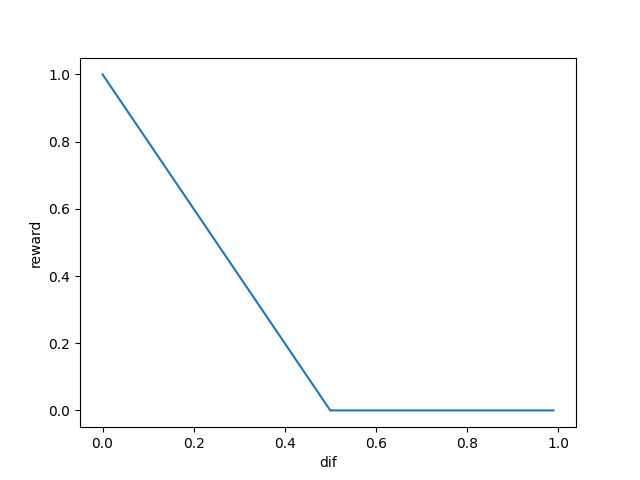
\includegraphics[width=0.35\textwidth]{reward_func.png}
	\caption{\label{fig:reward_func}Iteration step reward based on the difference between estimated and true source value.}
\end{wrapfigure}
%
Thus, the rewards are in the interval $[0,1]$. As you can see in fig. (\ref{fig:reward_func}) the reward decreases linearly based on the difference between the estimated and the real true source value. If the difference is larger than $0.5$ or all members of the network are excluded the reward is $0$. Note that there is no punishment for excluding members from the social network. Therefore, a solution with a lot of exclusions might still be considered good independent from wether the exclusions were justified or not. Although this might be problematic in some real world applications minimizing the number of exclusions is not in the scope of this work. \newline

The social network environment as described in section (\ref{sec:SN}) and (\ref{sec:SN_RLEnv}) was implemented as an OpenAI Gym \cite{gym} environment which yields the advantage of making the implementation compatible with many reinforcement learning frameworks.

\section{Training an agent with A2C}
Advantage Actor Critic (A2C) \cite{A2C_1} is a synchronous and deterministic variant of Asynchronous Advantage Actor Critic (A3C) \cite{A3C_1,A3C_2}. The idea of A3C is to train multiple workers simultaneously which all have an own version of a global network. Each worker has an own set of the network parameters and trains them separately on different copies of the environment. The workers then update the global network in an asynchronous way. This yields the advantage of having workers explore different regions of the environment which leads to more stable results. A2C doesn't asynchronously update the workers but instead waits until all workers are finished with their exploration step. The global model is then updated by averaging over all workers. This means that their is only one version of network parameters but each worker has an own environment to train on. While A3C has the advantage of fast training on CPU-based implementations \cite{A3C_1} - as each worker can run in a separate thread - A2C performs better with larger batch sizes and is thus better suited for GPU-based implementations. According to an OpenAI block post A2C yields more stable results than A3C \cite{A2C_3}. A2C is well suited for the introduced social network environment as it can handle large, continuous action and observation spaces \cite{A2C_1}. I used the stable baseline \cite{stable-baselines} implementation of A2C to train an agent with the environment introduced in the previous section. \newline
The next section gives a more detailed description of the Advantage Actor Critic method.

\subsection{Advantage Actor Critic}
The goal of a reinforcement learning agent is to find a policy $\pi$ that maximizes a reward function $g$ \cite{A2C_2}. Let us assume that the policy $\pi$ is parameterized with parameters $\theta$. Often $g$ is defined as the expected discounted sum of rewards where future rewards are discounted by a factor $\gamma$
%
\begin{equation}
	g(\theta) = \mathbb{E}[\sum_{i}^{} \gamma^i r_{i+1}]
\end{equation}
%
This is also useful in the scenario of finding misinformation in social networks as the longer members with false beliefs stay in the network the more their propagated misinformation can spread into the network. Thus, rewards in early iterations are more important than rewards in later iterations.\newline
In order to find the maximum of $g(\theta)$ with gradient ascent the gradient $\nabla_\theta g(\theta)$ has to be used to update the parameters, that is
\begin{equation}
\theta' = \theta + \nabla_\theta g(\theta)
\end{equation}
The gradient of $g(\theta)$ for $N$ samples with $T$ iterations is 
\begin{equation} \label{equ:pol_grad}
	\nabla_\theta g(\theta) \approx \frac{1}{N} \sum_{i=1}^{N}\sum_{s=1}^{T}\nabla_\theta \log \pi_\theta(a_{s,i}|x_{s,i}) \left(\sum_{s'=1}^{T}\gamma^{s'} r(s_{s',i},a_{s',i})\right)
\end{equation}
A detailed derivation of the gradient can be found at \cite{pol_grad2, pol_grad1}. Let us now take a look at the state value function and the state-action value function.
The state value function is defined as the expected sum of future rewards given an initial state $x_0$ and a policy $\pi$
%
\begin{equation}
	V^{\pi}(x_0)=\mathbb{E}[\sum_{t=0}^{\infty}\gamma^tr(x_t,a_t)|a_t\sim\pi_t]
\end{equation}
%
It is also called V value. In contrast to that the state-action value function or Q-value is directly dependent on a given action $a$ instead of sampling $a$ from a policy $\pi$. The state-action value function can be defined as 
%
\begin{equation}
\begin{split}
	Q^\pi(x_i,a_i) 
		& =\mathbb{E}[r(x_i,a_i)+\gamma V^{\pi}(x_{i+1})] \\
		& =\mathbb{E}[\sum_{t=0}^{T} \gamma^t r(x_t,a_t)| x_0=x_i, a_0=a_i, a_{t+1} \sim \pi_{\theta}]
\end{split}
\end{equation}
%
where action $a_i$ leads to a transition from state $x_i$ to state $x_{i+1}$. After action $a_i$ it is assumed that the agent again follows the policy $\pi$. As you can see does the second term of equation (\ref{equ:pol_grad}) correspond to the Q-value. It can thus be written as
\begin{equation}
	\nabla_\theta g(\theta) \approx \frac{1}{N} \sum_{i=1}^{N}\left[\sum_{s=1}^{T}\nabla_\theta \log \pi_\theta(a_{s,i}|x_{s,i}) Q(s_t,a_t)\right]
\end{equation}
Practice has shown that it is more stable to use the advantage term instead of directly using Q-values \cite{A3C_1}. The advantage term defines how much better it is to take a certain action $a_t$ compared to other actions given a state $x_t$, that is
%
\begin{equation}
\begin{split}
A^\pi(x_t,a_t) & = Q^\pi(x_t,a_t) - V^\pi(x_t) \\
& = r(x_t,a_t) + \gamma V^{\pi}(x_{t+1}) - V^{\pi}(x_{t})
\end{split}
\end{equation}
%
The resulting update term of A2C is then
\begin{equation} \label{equ:pol_grad_fin}
	\nabla_\theta g(\theta) \approx \frac{1}{N} \sum_{i=1}^{N}\left[\sum_{s=1}^{T}\nabla_\theta \log \pi_\theta(a_{s,i}|x_{s,i}) A^\pi(x_{s,i},a_{s,i})\right]
\end{equation}
The basic idea of actor-critic methods is to have an actor who tries to find an optimal policy $\pi$ and a critic that tries to estimate the value function. Both are parameterized with neural networks. Note that the advantage can directly be calculated from the estimated value function of the critic and the returned rewards during training. Equation (\ref{equ:pol_grad_fin}) can then be used to iteratively update the parameters of the actor an the critic network. \newline
%
\subsection{Entropy in Advantage Actor Critic}
In reinforcement learning it is often beneficial to add the policy entropy to the objective function \cite{entropy_1}. Policies with high entropy are often sub-optimal deterministic policies \cite{A3C_1}. Adding the policy entropy to the objective function penalizes those kinds of policies and thus encourages exploration . For the environment described in section (3) we know that an optimal policy has to have a low entropy as nodes which are trustworthy or not trustworthy are in a random order in each run. Therefore adding the policy entropy to the object function further improves the convergence to an optimal solution. Following \cite{A3C_1} the full gradient of the objective function then is
\begin{equation}
	\label{equ:pol_grad_fin}
	\nabla_\theta g(\theta) \approx \frac{1}{N} \sum_{i=1}^{N}\left[\sum_{s=1}^{T}\nabla_\theta \log \pi_\theta(a_{s,i}|x_{s,i}) A^\pi(x_{s,i},a_{s,i}) + \beta \nabla_\theta H(\pi_\theta(x_{s,i}))\right]
\end{equation}
where $H$ is the entropy and $\beta$ is a hyperparameter which controls how much the entropy term influences the objective function. In the following $\beta=0.04$.

\subsection{Network Architecture}
As mentioned before both the actor and the critic are parameterized with neural networks. Different network architectures are conceivable. One interesting idea would be to use graph neural networks (GNNs) \cite{gnn_1, gnn_2, gnn_3} which can incorporate the topology of a graph and are thus inherently suitable for learning in social networks. Combining reinforcement learning with GNNs is a fairly new research topic \cite{rl_gnn2, rl_gnn1} and I thus decided against using it as it would exceed the scope of this project. \newline

%
\begin{wrapfigure}{R}{0.41\textwidth}
	\centering
	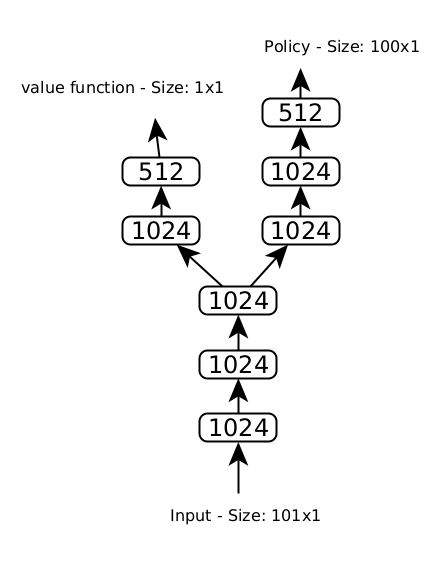
\includegraphics[width=0.41\textwidth]{NN_architecture.png}
	\caption{\label{fig:NN_arch}Network architecture for the actor and the critic. Both share the first 3 layers. The numbers in the layers indicate amount of nodes. All layers are fully connected.}
\end{wrapfigure}
%

Another idea is to use long short-term memory (LSTM) networks in order to account for the time dependency between two consecutively states. I found that for this scenario LSTM networks don't yield better results but need much longer to train. Therefore, I decided to use fully connected multilayer perceptrons (MLPs). The layer structure for a social network with 100 nodes and 10 external sources is shown in figure (\ref{fig:NN_arch}). The actor and critic share the first 3 layers. This reduces the training time as fewer parameters have to be trained. It also leads to more stable results as in the first 3 layers a good generalization of the input has to be learned as the output is used to calculate both the value function as well as the policy. During the tuning of the network parameters I found that for this scenario multiple layers work better than fewer layers with more nodes. The $\tanh$ function is used as an activation function in order to address the vanishing gradient problem. The optimizer used in the stable-baselines implementation of A2C is RMSprop \cite{RMSprop}.

\subsection{Pre-Training}
Achieving convergence to an optimal solution is often hard in reinforcement learning \cite{rlblogpost}. Pre-training the agent was a crucial part in this work in order to achieve good results. Pre-training in the context of reinforcement learning is basically training the actor in a supervised fashion with a dataset created by an expert. In this scenario the action of this expert for each node $i$ at time $t$ is defined as
%
\begin{equation}
	a_{\text{expert}}(s_i(t)) = \begin{cases}
			1 & |s_i - s_T| < 0.1 \\
			0 & |s_i - s_T| > 0.3 \\
			0.5 & \text{otherwise}
		\end{cases}
\end{equation}
%
Note that in contrast to the reinforcement learning agent this expert has knowledge of the true source value $s_T$. During the pre-training phase first a dataset is created where the expert agent interacts with the environment. Then the actor is trained with those state-action pairs in a supervised fashion. The critic is not trained during this phase but it indirectly benefits due to the 3 shared layers. The purpose of the pre-training phase is to give a better initialization of the network parameters in order to get better and more stable results. A deeper analysis of the effect of the pre-training phase can be found in the next section.


\section{Results}
In this chapter a social network with 100 nodes, 10 external sources and a connectivity of $p_c=0.1$ run for 10 iterations is evaluated. Although a social network with 100 nodes might seem small it wasn't possible for me to scale up the nodes further due to limited hardware resources. The discount factor for rewards is $\gamma=0.99$. In order to evaluate the performance of the reinforcement learning agent a do-nothing agent is used as a baseline. This agent doesn't excluded any members of the network and just gives every node full trust. Note that due to the normalization in equation (\ref{equ:s_est}) the exact trust value doesn't influence the rewards as long as the agent gives every node the same trust and doesn't exclude any node. This agent has the same performance as an agent that assigns random trust values without excluding all members of the network. \newline
In the following sections an agent is pre-trained on 600k samples and then A2C is run for 5 millions total iterations.

\subsection{Performance for varying Levels of Misinformation}
In this section the performance of the agent is evaluated for different levels of misinformation in the network, that is a different ratio of true and false sources. You can find the results for the baseline do-nothing agent the pre-trained model without reinforcement learning and the fully trained model in table \ref{tab:perf_1}. All 3 agents are run 300 times over different initializations of the environment. Thereby the environments are initialized with the same seed for all 3 agents as there is quiet a high variance between multiple runs.

\begin{center} \label{tab:perf_1} 
	\scalebox{0.88}{
	\begin{tabular}{ m{6em} | m{5em} | m{5em} | m{5em}}
								   & do-nothing agent & pre-training only & complete model \\
								   \hline
		1 true and 9 false sources & 1.09			  & 1.46			  & 1.49 \\
		\hline
		2 true and 8 false sources & 1.68			  & 2.52			  & 2.70 \\
		\hline
		3 true and 7 false sources & 2.57		      & 3.77			  & 3.89 \\
		\hline
		4 true and 6 false sources & 3.45			  &	4.62			  & 4.60 \\
		\hline
		5 true and 5 false sources & 4.46			  & 5.01			  & 5.0 \\
		\hline
		6 true and 4 false sources & 5.30			  & 5.96			  & 6.35 \\
		\hline
		7 true and 3 false sources & 6.47			  & 7.26			  & 7.31 \\
		\hline
		8 true and 2 false source  & 7.39			  &	8.19			  & 8.26 \\
		\hline
		9 true and 1 false source  & 8.43			  &	8.70			  & 8.69
	\end{tabular}} 
	\captionof{table}{Discounted rewards for the baseline do-nothing agent, the pre-trained model and the fully trained, complete model for different ratio of true and false sources. Mean value over 300 runs.}
\end{center}

As you can see the fully trained model performance better for all ratios of false and true sources. The maximum possible reward for each run is 
\begin{equation}
	r_\text{max} = \sum_{t=1}^{10} 0.99^t \approx 9.56
\end{equation}
as the maximum reward for each iteration is $1$. In figure \ref{fig:per_cm} the do-nothing agent and the fully trained model are directly compared.

\begin{figure}[h] 
	\centering
	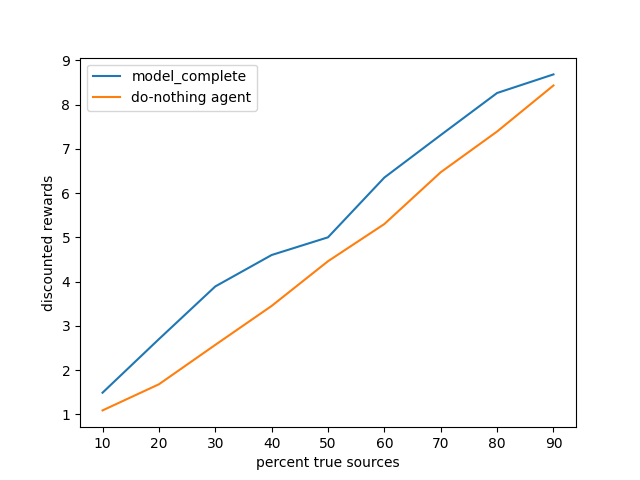
\includegraphics[width=0.55\textwidth]{perf_cm.png} 
	\caption{\label{fig:per_cm} Comparison between the fully trained model and the do-nothing agent for different ratios of true and false sources.}
\end{figure}

Although the fully trained model outperforms the do-nothing agent for all ratios of misinformation the total discounted rewards decrease linearly for both agents for an increasing amount of false sources. The difference between the two agents remains roughly at $1$. In order to understand how it is even possible for the fully trained agent to get a better performance for the case with only $1$ true source one has to keep in mind that $|s_\text{true}-s_\text{false}| > 0.3$ for all false sources. This means that for few false sources the agent has to assign low trust values to nodes with outlier belief values and in the case of few true sources the agent has to assign high trust values to nodes with outlier belief values. This type of outlier detection becomes harder for the case of a majority of false sources as the false sources have different belief values. This might be one reason why the rewards decrease for a higher percentage of ratio sources. The constant difference between do-nothing agent and fully trained agent also indicates that the fully trained agent cannot fully minimize the spread of misinformation but rather decreases it by the same degree for different ratio of true and false sources. A deeper analysis of the behavior of the agent can be found in section \ref{sec:res_behavior}. \newline

\begin{figure}[h]
	\centering
	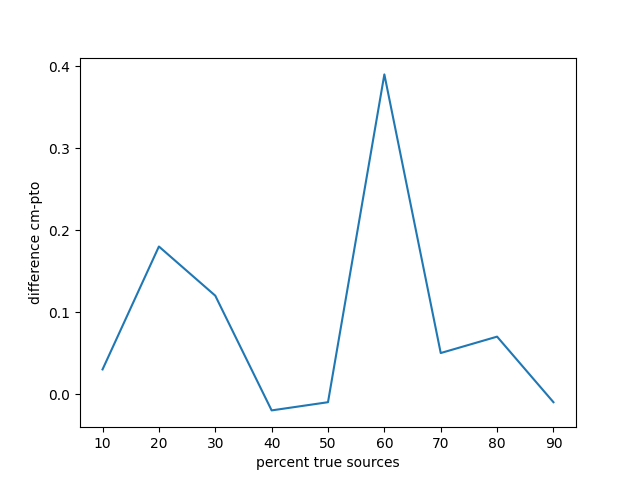
\includegraphics[width=0.55\textwidth]{dif_cm-pto.png}
	\caption{\label{fig:dif_cm-pto} Difference between pre-trained model and fully trained model for different ratio of false and true sources.}
\end{figure}

In figure \ref{fig:dif_cm-pto} you can find the difference between pre-trained and fully trained model. As you can see the fully trained model performs significantly better than the only pre-trained model for 7 out of 10 ratios. For 3 out of 10 ratios the two models almost performed the same, meaning that the reinforcement learning part didn't increase the returned rewards. The difference between the two model and the ratio between true and false sources doesn't seem to correlate. This indicates that the agent gets stuck in local maxima.

\subsection{Behavior of Trained Agent} \label{sec:res_behavior}
In this section the behavior of the fully trained agent is investigated by looking at what action the agent chooses for certain observations. The observation action pair for 7 true and 3 false sources for the first 10 nodes are shown in figure \ref{fig:act-obs_7t3f}.

\begin{figure}[h]
	\begin{subfigure}{\textwidth}
		\centering
		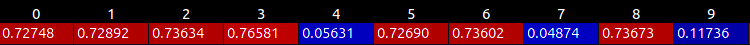
\includegraphics[width=.85\linewidth]{7t3f_obs_iter1_hc.png}  
		\caption{Belief value of first 10 nodes.}
	\end{subfigure}
	\begin{subfigure}{\textwidth}
		\centering
		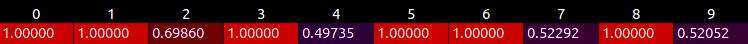
\includegraphics[width=.85\linewidth]{7t3f_action_iter1_hc.png}  
		\caption{Action for first 10 nodes.}
	\end{subfigure}
	\caption{\label{fig:act-obs_7t3f}First part of observation and corresponding action of the fully trained agent. There are 7 true and 3 false sources. This observation was created in the first iteration. Only the first 10 of 100 values are shown.}
\end{figure}

As you can see do nodes at index 4 and 7 propagate the belief value of a false source, node 9 propagates the belief value of a different false source and the remaining nodes propagate the belief of the true source. The agent correctly assigns the lowest trust values to the 3 nodes that propagate false belief values but it doesn't exclude the nodes. The nodes that propagate true belief values all get maximum trust values with the exception of node 2 that incomprehensibly also gets a relative low trust value. This example illustrates that the behavior of the agent goes into the right direction but is not fully optimal. This again indicates convergence to a local maxima. \newline

The next example in figure \ref{fig:act-obs_3t7f} shows the observation action pairs for 7 false and 3 true sources for 2 iterations. The true source value is $s_T = 0.10$.

\begin{figure}[h]
	\begin{subfigure}{\textwidth}
		\centering
		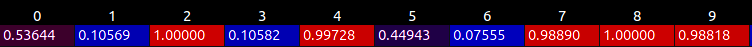
\includegraphics[width=.85\linewidth]{3t7f_obs_iter1_hc.png}  
		\caption{Observation in iteration 1}
		\label{fig:3t7f_obs_iter1}
	\end{subfigure}
	\begin{subfigure}{\textwidth}
		\centering
		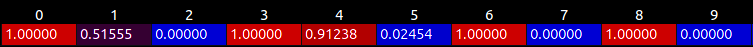
\includegraphics[width=.85\linewidth]{3t7f_action_iter1_hc.png}  
		\caption{Action in iteration 1}
		\label{fig:3t7f_action_iter1}
	\end{subfigure}
	\begin{subfigure}{\textwidth}
		\centering
		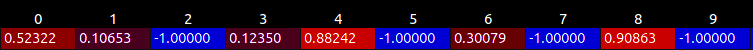
\includegraphics[width=.85\linewidth]{3t7f_obs_iter2_hc.png}  
		\caption{Observation in iteration 2}
		\label{fig:3t7f_obs_iter2}
	\end{subfigure}
	\begin{subfigure}{\textwidth}
		\centering
		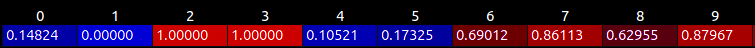
\includegraphics[width=.85\linewidth]{3t7f_action_iter2_hc.png}  
		\caption{Action in iteration 2}
		\label{fig:3t7f_action_iter2}
	\end{subfigure}
	\caption{\label{fig:act-obs_3t7f}Observation and corresponding action for 2 iterations. There are 7 false and 3 true sources. The true source value is $s_T=0.10$.}
\end{figure}

As you can see nodes with indices 1,3 and 6 propagate true belief values and the other nodes propagate false belief values. The agent excludes nodes 2,5,7 and 8 from the network. All those nodes propagate false belief values. Besides that nodes with true and false source values get high and low trust values. Nodes 2,4,7,8 and 9 all propagate a false belief value close to $1$ but while nodes 2,7 and 9 get excluded from the network nodes 4 and 8 surprisingly get a high trust value. In the observation for the next iteration in figure \ref{fig:3t7f_obs_iter2} it is possible to see that misinformation leaked into the network. From the 3 nodes that propagated true belief values in the previous iteration only one (node 1) still has a belief value that is close to the true one. Especially node 6 heavily changed its belief value. The action of the agent looks rather random. Note that the belief value for excluded nodes has no influence. \newline
This example confirms that the agent doesn't act fully optimal which again indicates convergence to a local maxima. This might be caused by multiple reasons. It wasn't possible for me to do a full hyperparameter search due to limited hardware resources. Increasing the network complexity of the actor and the critic could also improve the performance as well as training for more iterations. In the next section a deeper insight into the convergence behavior is given.

\subsection{Convergence}
6t4f
\begin{figure}[h]
	\begin{subfigure}{0.45\textwidth}
		\centering
		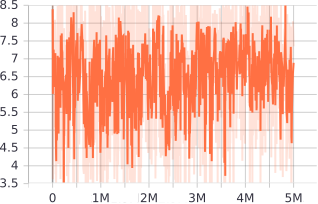
\includegraphics[width=\linewidth]{reward_notSmoothed.png}  
		\caption{.}
	\end{subfigure}
	\begin{subfigure}{0.45\textwidth}
		\centering
		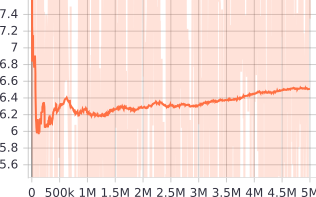
\includegraphics[width=\linewidth]{reward_smoothed.png}  
		\caption{.}
	\end{subfigure}
	\caption{\label{fig:reward_tb}.}
\end{figure}

\begin{figure}[h]
	\begin{subfigure}{0.45\textwidth}
		\centering
		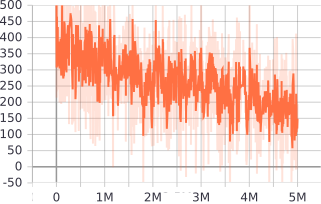
\includegraphics[width=\linewidth]{loss_notSmoothed.png}  
		\caption{.}
	\end{subfigure}
	\begin{subfigure}{0.45\textwidth}
		\centering
		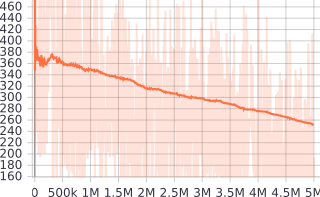
\includegraphics[width=\linewidth]{loss_smoothed.png}  
		\caption{.}
	\end{subfigure}
	\caption{\label{fig:loss_tb}.}
\end{figure}

\section{Conclusions}


\clearpage
\bibliography{references}{}
\bibliographystyle{plain}
\end{document}